\documentclass[11pt]{report}
\usepackage[utf8]{inputenc}
\usepackage[T1]{fontenc}
\usepackage[english]{babel}
\usepackage{graphicx, caption, subcaption}
\usepackage{geometry}
\usepackage{xcolor}
\usepackage{listings}
\usepackage{hyperref}
\usepackage{float}
\usepackage{csquotes}
\usepackage{csvsimple}
\usepackage{parskip}
\usepackage{booktabs}
\usepackage{array}
\usepackage{afterpage}
\usepackage{tcolorbox}
%\usepackage[
%backend=biber,
%style=alphabetic,
%sorting=ynt
%]{biblatex}
%\addbibresource{bibliography.bib}

% \usepackage[document]{ragged2e}

\geometry{
    a4paper,
    tmargin = 2.5cm,
    bmargin = 2.5cm,
    lmargin = 2.5cm,
    rmargin = 2.5cm
}

\hypersetup{
    colorlinks = true,
    linkcolor = black,
    filecolor = olive,      
    urlcolor = olive,
    citecolor = olive
}

\definecolor{codegreen}{rgb}{0,0.6,0}
\definecolor{codegray}{rgb}{0.5,0.5,0.5}
\definecolor{codepurple}{rgb}{0.58,0,0.82}
\definecolor{backcolour}{rgb}{0.92,0.92,0.92}

\lstdefinelanguage{C}{
      morekeywords={
        SCCResult,ListGraph,SubGraph
      },
      morecomment=[l]{//}, 
      morecomment=[s]{/}{/},
      breaklines=true,
      numbers=left,
      captionpos=b,
      breakatwhitespace=true,
      basicstyle=\linespread{1.0}\ttfamily\small, 
}
    
\lstdefinestyle{CodeStyle}{
    backgroundcolor=\color{backcolour},   
    commentstyle=\color{codegreen},
    keywordstyle=\color{magenta},
    numberstyle=\tiny\color{codegray},
    stringstyle=\color{codepurple},
    basicstyle=\ttfamily\small,
    breakatwhitespace=false,         
    breaklines=true,                 
    captionpos=b,                    
    keepspaces=true,                 
    numbers=left,                    
    numbersep=5pt,                  
    showspaces=false,                
    showstringspaces=false,
    showtabs=false,                  
    tabsize=2,
    escapechar={|}, 
    language=bash
}
\lstset{style=CodeStyle}

\begin{document}

\begin{titlepage}

    \begin{minipage}[b]{0.3\textwidth}
        \begin{flushleft}
            
\includegraphics[width=5cm]{assets/unisa.png}
        \end{flushleft}
    \end{minipage}
    \hfill
    \begin{minipage}[b]{0.7\textwidth}
        \begin{flushright}
            \raggedleft{DIEM - University of salerno}
                \\ Master's degree in Computer Engineering
                \\ Situation Awareness
        \end{flushright}
    \end{minipage}

    \hrulefill

    \vspace{1cm}

    \begin{LARGE}
        \raggedleft\textbf{Project Report}
    \end{LARGE}

    \begin{large}
         
    \end{large}

    \vspace{1.0cm}

    \begin{minipage}[t]{7cm}
        \flushleft
        \textsc{Lecturers:}\\
        \textit{Giuseppe D'Aniello,}\\ 
        \textit{Matteo Gaeta}\\
    \end{minipage}

    \vspace{0.5cm}
    
    \textsc{Group Members:}\\
    \begin{table}[h!]
        \centering
        \begin{tabular}{| m{3cm} | m{3cm} | m{3cm} | m{6cm} |}
        \hline
        \textbf{Surname} & \textbf{Name} & \textbf{Number} & \textbf{E-mail} \\ 
        \hline
        Galasso & Gianluca & 622702000 & g.galasso33@studenti.unisa.it \\ 
        \hline
        Iovaro & Damiana & 622702017 & d.iovaro@studenti.unisa.it \\ 
        \hline
        Murati & Camilla & 622702126 & c.murati@studenti.unisa.it \\ 
        \hline
        Sellitto & Marco & 622702105 & m.sellitto13@studenti.unisa.it \\ 
        \hline
        \end{tabular}
        \label{table:1}
    \end{table}

\end{titlepage}


\tableofcontents

\chapter[Introduction]{Introduction}\label{ch:introduction}
The objective of this project is to implement a comprehensive e-learning system designed to assist users 
in tailoring their learning pathways and enhancing their skill sets. Developed with a strong emphasis on 
situational awareness, this project is structured into two primary components: the first involves 
\textit{Goal-Driven Task Analysis} (GDTA), and the second focuses on the implementation of an integrated dashboard.

This system is meticulously crafted with a \textbf{User-Centric Approach}, ensuring that users can effectively 
monitor their competencies and track their learning progress. In developing the GDTA, we delineated operational 
concepts through detailed personas and scenario analysis, ensuring that the system is attuned to the diverse needs 
and contexts of its users. To fulfill the goals described inside the GDTA, we implemented two dashboards: the first
dashboard is focused on the user's global learning progress, while the second dashboard is focused on the user's
progression in a specific course.

For the dashboard implementation, we leveraged \textit{ElasticSearch} as the underlying database and \textit{Kibana} 
as the visualization tool. The data presented on the dashboard were specifically curated for this project and are 
stored in multiple .csv files. 

Initially, our goal was to conduct a comprehensive data analysis using an extensive dataset found online. However, 
we faced significant challenges in locating suitable data that aligned perfectly with our needs. Consequently, we 
chose to create our own .csv files containing the essential data required to populate our dashboard. 
This decision granted us full control over the data, enabling precise customization according to the specific 
requirements of our project. By curating our own dataset, we ensured the accuracy and relevance of the information 
presented, thereby facilitating a more insightful and effective implementation of our e-learning system. The data 
are shown on a time slice of twenty days, from the first of May to the twentieth of May. The reason for 
this time interval is to illustrate the user's learning situation on the platform before the end of the courses,
which is set for the last day of May. 



\chapter[Data Description]{Data Description}\label{ch:data-description}
The dataset used to create the mockup of the dashboards has been handcrafted by the authors.
It consists of different CSV files, each one representing a table. These files describe
the courses within an e-learning platform, the interactions between a user and courses,
the interactions between users, the resources used by the user on the platform, and the user's
results in the courses.

The dataset is composed of the following tables:
\begin{itemize}
    \item 
        \textbf{Completed Course:} This table indicates whether the user has completed something each 
        day or not for the different courses;
    \item 
        \textbf{User Hours Sessions:} This table represents the hours spent by the user on the platform 
        each day and the average hours spent by other users;
    \item 
        \textbf{Resources:} This table represents the hours of use of the different resources that are
        available on the platform for each day;
    \item 
        \textbf{Forum:} This table represents the interactions between users on the forum, showing the number
        of questions asked, the number of answers given, and the number of answers received;
    \item 
        \textbf{Completed Modules Votes:} This table shows the votes obtained by the user for each completed module, 
        categorized by type (theory or exercise).
\end{itemize}

The files produced are tailored on the specific dashboard where used. Some of the previously described files
are duplicated and adapted to the particular needs of the dashboard. For example, the \textit{Forum} table describes
the interactions for each course or the interactions for each module inside a specific course. The same applies to the
\textit{Resources} table, where the resources are divided by course or represent the resources used for a particular course.


\chapter[Operational Concept]{Operational Concept}\label{ch:operationalconcept}
We questioned which requirement could be critical for a Situational Awareness System. This phase involved identifying and understanding the essential needs that the system must fulfill to be effective and user-friendly. 

To achieve this, we conducted a detailed analysis of the \textit{Operational Concept}, which involved the development of detailed personas and scenario analysis. 

The Operational Concept is a critical phase in the design of complex systems, translating system requirements into actionable plans. 
It provides a comprehensive understanding of the system's operational environment, including the roles and responsibilities of the users, the tasks they perform, and the context in which they operate.

Since we are developing an e-learning dashboard intended for users who may access it from various locations, we have not defined specific environmental constraints. The flexibility of online learning environments means that users could be utilizing the system in diverse settings, such as homes, offices, or public spaces, each with varying levels of connectivity and hardware capabilities.

\section{Scenario}
The company requires all employees to pursue upskilling or reskilling opportunities based on their previous studies and work experiences. Marta and Matteo are two employees whose skills and knowledge will be monitored to ensure they can effectively contribute to projects in the Offensive Cybersecurity field. The company’s e-learning platform provides courses that enable employees to obtain the \textit{OSCP} (Offensive Security Certified Professional) certification.

The platform is accessible both on-site at the company and remotely, offering flexible learning options that accommodate diverse schedules. Each employee receives a personalized dashboard where they can track their progress and access a wide range of educational resources, including video courses (concept pills), slide decks, and practical exercises. At the end of each module, employees can take assessments to reinforce their understanding and ensure they meet the learning objectives.

Additionally, the platform includes analytics and trend reports that help employees understand their learning journey, estimate the time required for course completion, and measure their engagement levels. The course design features a tailored approach, continuously monitoring each employee’s performance and adapting to their specific learning needs. This customization enhances the overall learning experience, ensuring employees are well-prepared for the OSCP certification.

\section{Supported Figure: Matteo}
Matteo is a student from the University of Salerno, with a bachelor's degree in Computer Engineering. His passion for cybersecurity has led him to specialize in this field, acquiring basic skills ranging from understanding the fundamentals of cybersecurity to networking and network protocols, from vulnerability analysis to familiarity with essential security tools. Now, Matteo faces a new challenge: a project in collaboration with Marta concerning Offensive Cybersecurity. However, to best address this task, Matteo needs to broaden his skills and knowledge.

\begin{center}
    \begin{tabular}{|l|p{10cm}|}
    \hline
    \textbf{Characteristic} & \textbf{Description} \\
    \hline
    Age Range & 20-25 \\
    \hline
    Gender & Male \\
    \hline
    Culture & Italian \\
    \hline
    Education & Bachelor's degree in Computer Engineering \\
    \hline
    Language & Italian, English (proficient for technical literature) \\
    \hline
    Frequency of Use & Several times a week \\
    \hline
    Experience & Familiar with basic cybersecurity tools and platforms, intermediate programming skills \\
    \hline
    Personality & Curious, analytical, detail-oriented, enjoys problem-solving, goal-oriented, collaborative \\
    \hline
    Acquired Skills & Fundamentals of cybersecurity, networking, vulnerability analysis, basic scripting/programming, offensive cybersecurity \\
    \hline
    Learning Style & Visual and hands-on learner \\
    \hline
    \end{tabular}
    \end{center}
    
\newpage
\section{Supported Figure: Marta}
Marta is a student from the University of Naples Federico II. She completed a bachelor's degree in Computer Engineering and has now specialized in machine learning, acquiring basic skills in the field of artificial intelligence, including the structure and applications of neural networks and deep neural networks, their applications in robotics, and autonomous driving. Marta wants to collaborate with Matteo on a new project in the field of Offensive Cybersecurity. Since Marta has followed a different academic path from Matteo's, which does not involve cybersecurity, she needs to upskill her competencies.

\begin{center}
    \begin{tabular}{|l|p{10cm}|}
    \hline
    \textbf{Characteristic} & \textbf{Description} \\
    \hline
    Age Range & 20-25 \\
    \hline
    Gender & Female \\
    \hline
    Culture & Italian \\
    \hline
    Education & Bachelor's degree in Computer Engineering, specializing in Machine Learning \\
    \hline
    Language & Italian, English (proficient for technical literature) \\
    \hline
    Frequency of Use & A few times a week \\
    \hline
    Experience & Skilled in AI and Machine Learning platforms, novice in cybersecurity \\
    \hline
    Personality & Innovative, inquisitive, enjoys learning new skills, collaborative, adaptable \\
    \hline
    Acquired Skills & Basics of AI, neural networks, deep learning, robotics, autonomous driving, basic programming, willingness to learn cybersecurity \\
    \hline
    Learning Style & Visual and auditory learner, prefers structured guidance \\
    \hline
    \end{tabular}
    \end{center}

\chapter[Goal-Directed Task Analysis]{Goal-Directed Task Analysis}\label{ch:gdta}
We applied the \textit{Cognitive Task Analysis} (CTA) methodology to explore individuals' knowledge and thought processes. Among the various CTA methodologies available, we selected the \textit{Goal-Directed Task Analysis} (GDTA), specifically focusing on Situation Awareness (SA) and the goals inherent in SA processes. 

\section{Initial GDTA Goal Tree}
The initial GDTA Goal Tree, shown in Figure 4.1, identified three Major-Goals. However, after an in-depth review and analysis, we concluded that the Major-Goal 1 \textbf{"Identify prior knowledge in the field of Cybersecurity"} can be integrated into the Major-Goal 2 \textbf{"Define and evaluate the knowledge required for Offensive Cybersecurity by monitoring students' progress"}. This conclusion was drawn from a comprehensive analysis of the sub-goals associated with Major-Goal 1.

Upon examining the sub-goals of Major-Goal 1, it became evident that both the sub-goals and the Major-Goal itself address topics that students need to master throughout their learning journey in cybersecurity. Given that Major-Goal 2 aims to delineate the specific topics and skills students must acquire, we decided to incorporate Major-Goal 1 as a sub-goal within Major-Goal 2. This integration ensures a more cohesive framework for evaluating and defining the necessary knowledge for Offensive Cybersecurity. 

Furthermore, the sub-goals of Major-Goal 1 have been reclassified as Level 2 elements, signifying their importance in the comprehension phase of the learning process. 

\begin{figure}[H]
    \centering
    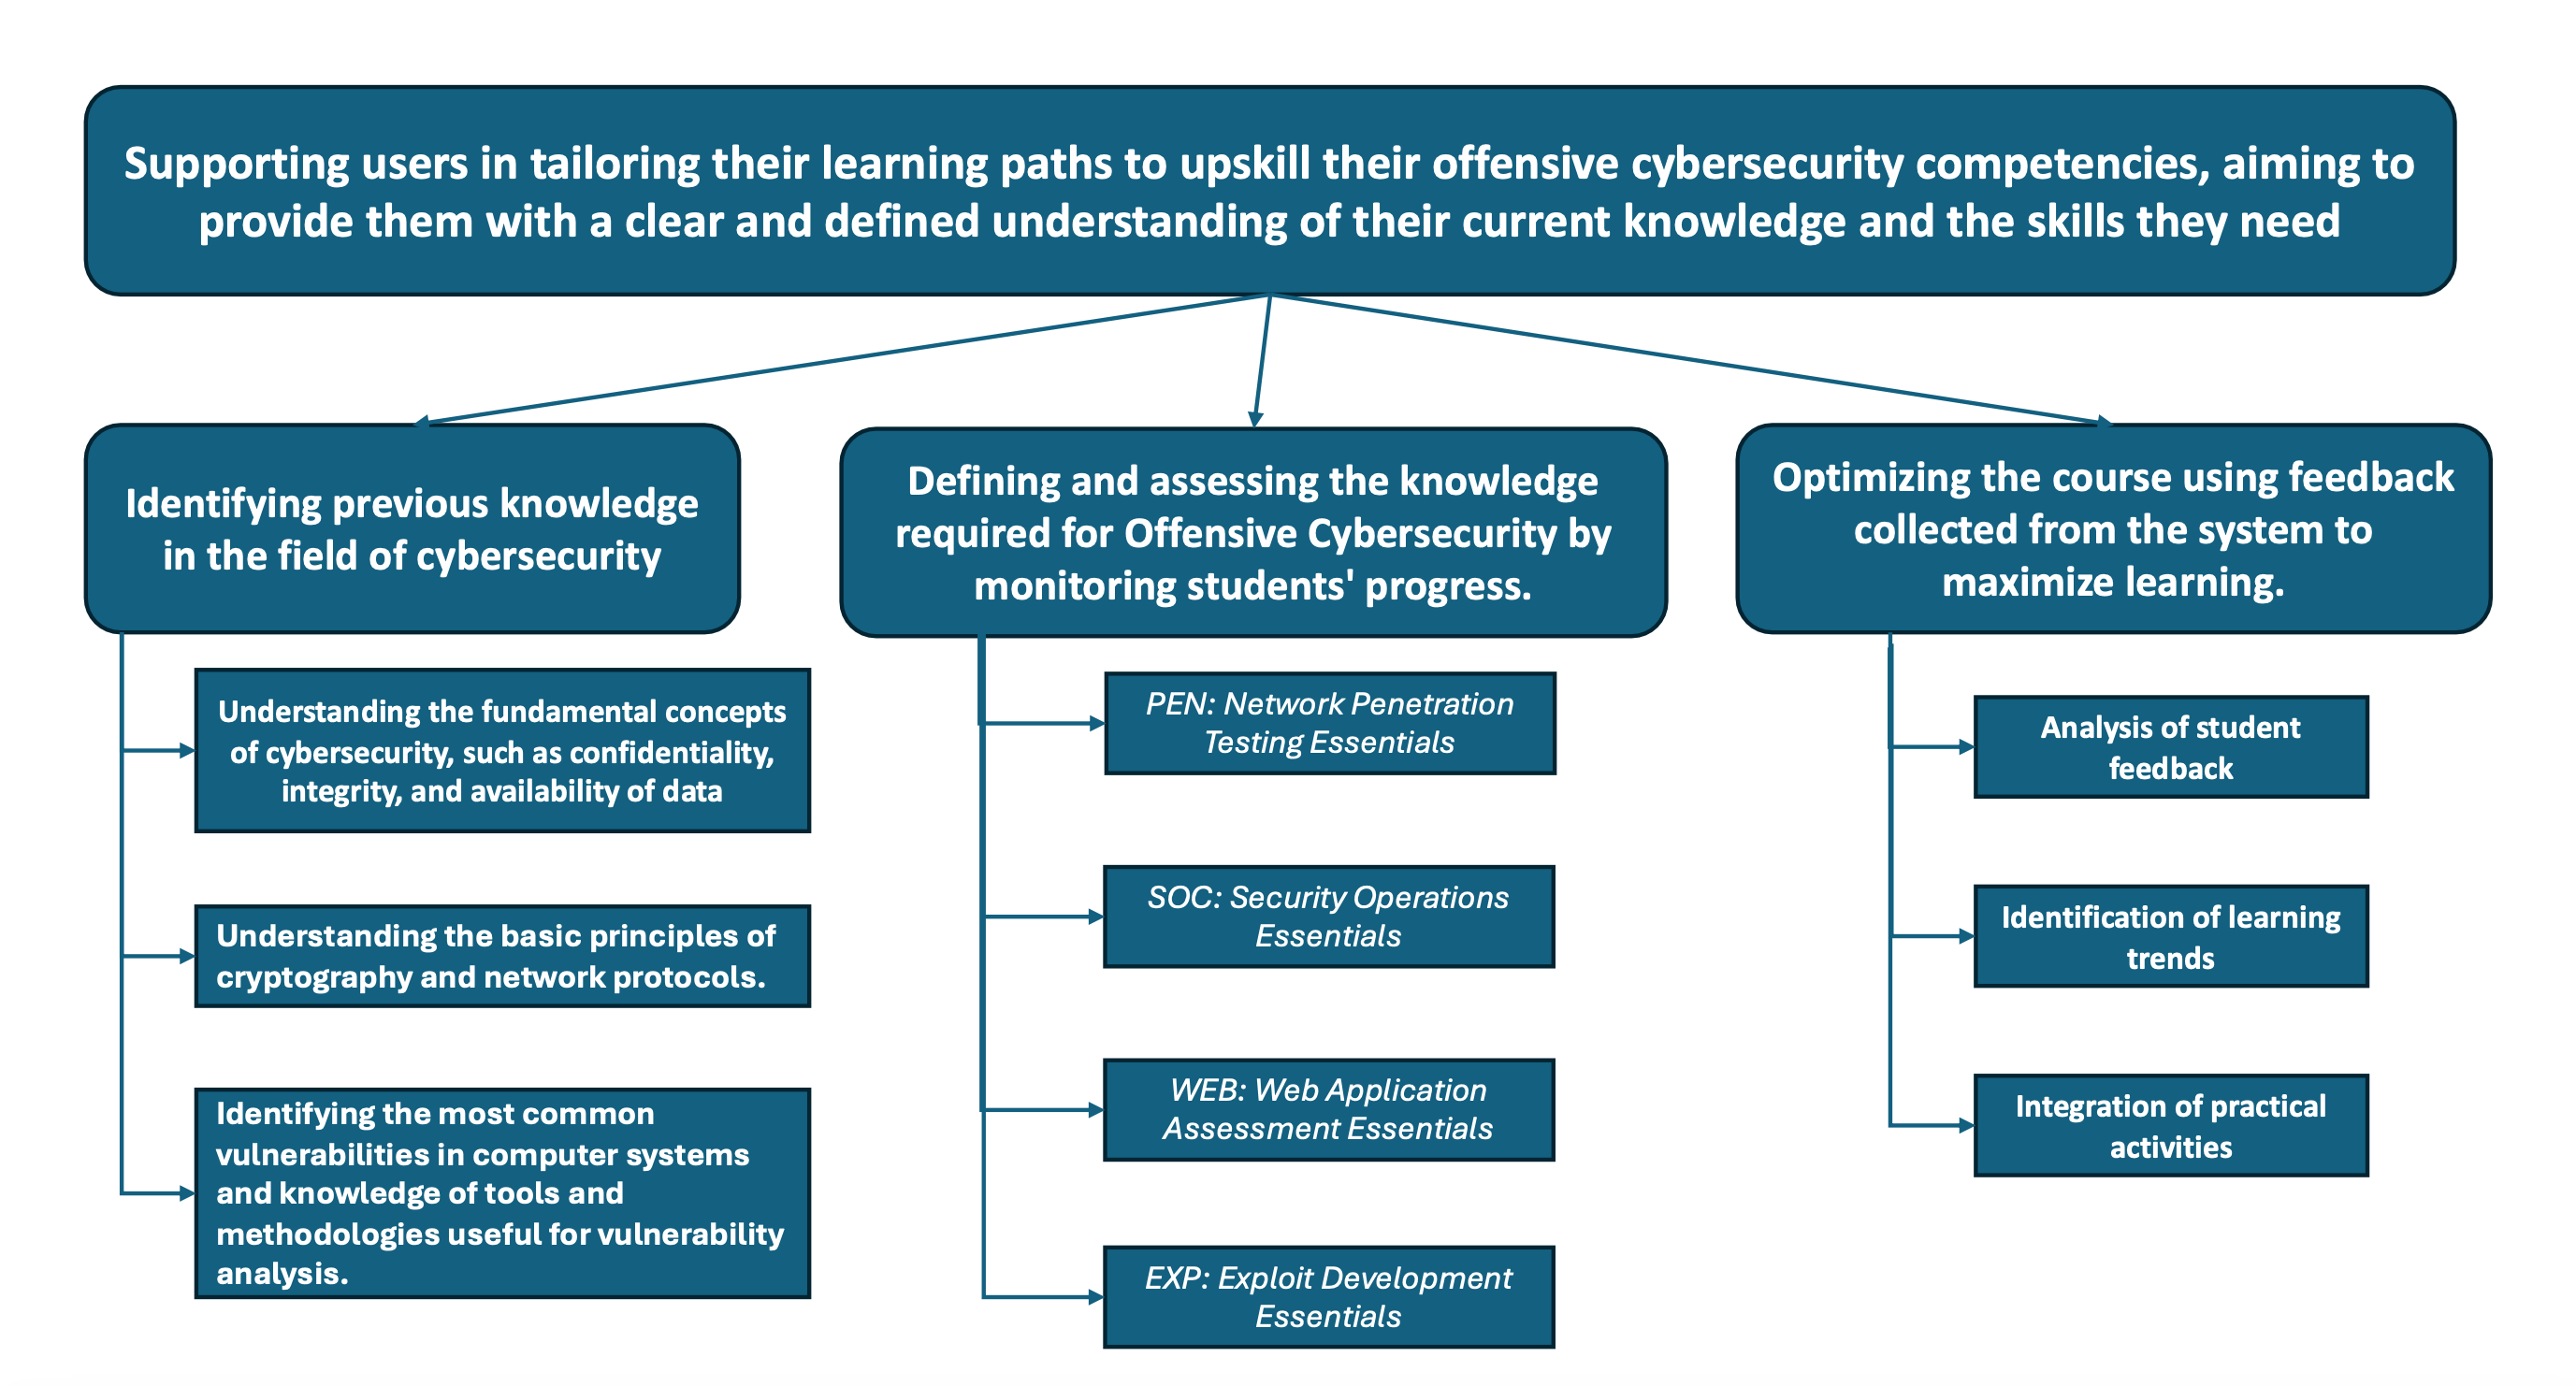
\includegraphics[width=\textwidth]{./assets/initialgdta.png}
    \caption{Initial GDTA Goal Tree}
    \label{fig:Initial GDTA}
\end{figure}

\newpage
\section{Final GDTA Goal Tree}
In Figure 4.2, we present our Final GDTA Goal Tree, which outlines the primary goals of the system and the sub-goals that contribute to their achievement. In particular, our GDTA Goal Tree supports users in adapting their learning paths to enhance their expertise in Offensive Cybersecurity.
The \textit{Overall Operator Goal} is broken down into two primary \textit{Major Goals} as shown in the picture below. Each Major Goal is further divided into \textit{SubGoals} that are essential for achieving the Major Goals. 

\begin{figure}[H]
    \centering
    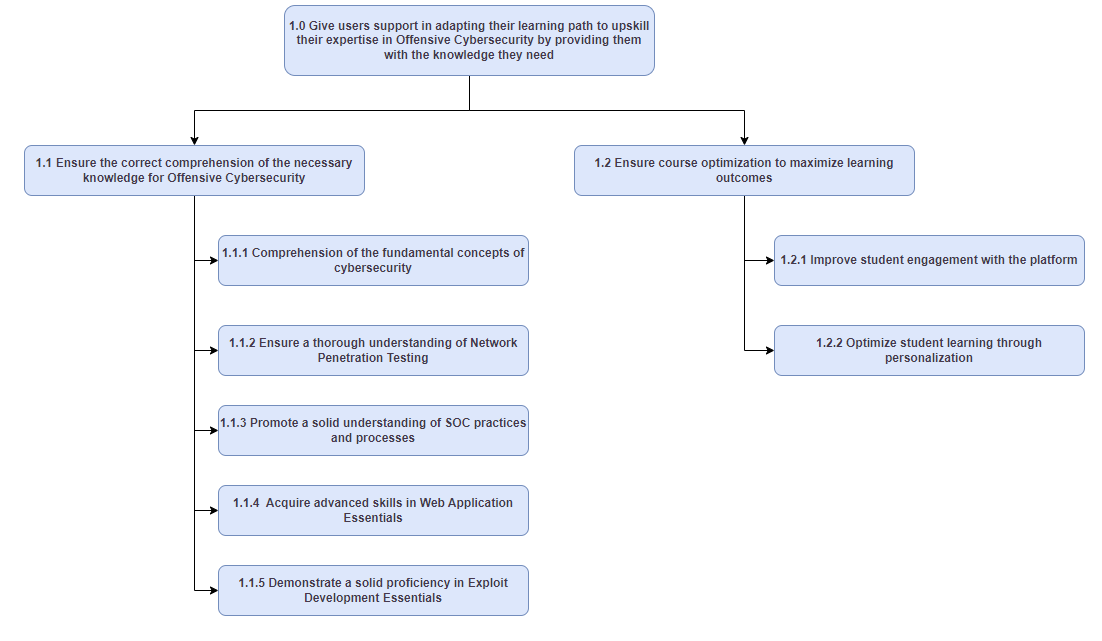
\includegraphics[width=\textwidth]{./assets/GDTA.png}
    \caption{Final GDTA Goal Tree}
    \label{fig:GDTA}
\end{figure}

The following sections will explain the details of each subgoal and their informational requirements, which are crucial for users to make informed decisions and achieve their objectives.
In order to fulfill a goal, a decision must be made based on the available information. We are not interested in trivial yes-or-no questions: instead, we are focusing on decisions that enable the fulfillment of high-level goals.

\newpage
\section{Major-Goal 1.1: Ensure the correct comprehension of the necessary knowledge for Offensive Cybersecurity}
In this section, we describe Major Goal 1.1 and its sub-goals.
The main aim of this goal, along with its sub-goals, is to outline the modules that users need to study to enhance their skills.

\subsection{Sub-Goal 1.1.1: Comprehension of the fundamental concepts of cybersecurity }
The objective of comprehending the fundamental concepts of cybersecurity is to provide individuals with a robust understanding of essential security principles and practices. Key areas of focus include ensuring confidentiality through mechanisms like OTP and MAC, maintaining data integrity with tools such as SHA256, and guaranteeing availability via digital signatures. Additionally, an understanding of blockchain technology and threat models is crucial, along with proficiency in cybersecurity algorithms and protocols like TLS. This foundational knowledge enables individuals to critically evaluate emerging technologies in relation to IT security and stay informed about current laws and regulations.

\begin{figure}[H]
    \centering
    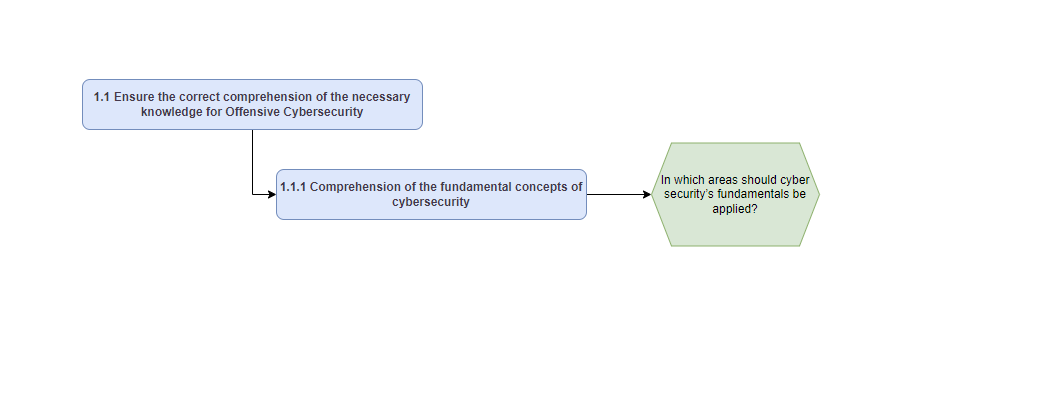
\includegraphics[width=\textwidth]{./assets/subgoal_1.1.1.png}
    \caption{Sub-Goal 1.1.1}
    \label{fig:subgoal_1.1.1}
\end{figure}

\begin{table}[H]
    \begin{center}
    \begin{tabular}{ | m{5cm} | m{5cm}| m{5cm} | } 
      \hline
      \textbf{Level 1 SA requirements} & \textbf{Level 2 SA requirements}  & \textbf{Level 3 SA requirements}  \\ 
      \hline
      CPA Security & Confidentiality & Capability to critically evaluate emerging technologies in relation to IT security, current laws and regulations\\ 
      \hline
      SHA256 & Integrity & \\ 
      \hline
      Advanced Schemes & Availability & \\ 
      \hline
      Zero Knowledge Proof &  Threat Models & \\ 
      \hline
      Blockchain & Algorithms for Cybersecurity  & \\ 
      \hline
      TLS Protocol &  & \\ 
      \hline
      Public Key&  & \\ 
      \hline
    \end{tabular}
    \end{center}
    \caption{SA requirements for subgoal 1.1.1}
    \end{table}
    
\newpage
\subsection{Sub-Goal 1.1.2: Ensure a thorough understanding of Network Penetration Testing}
The objective of ensuring a thorough understanding of network penetration testing is to equip individuals with the necessary skills and knowledge to effectively identify and mitigate security vulnerabilities within network infrastructures. This includes mastering fundamental programming concepts such as Python operators, syntax, and Powershell scripting, as well as understanding key network protocols like the Internet Protocol (IP) and Domain Name System (DNS). Advanced competencies involve applying cryptography techniques and hashing, acquiring in-depth Windows networking knowledge, and efficiently using variables, loops, and functions in Python and Powershell. Ultimately, this comprehensive understanding enables individuals to select the most appropriate penetration testing strategies for various scenarios, ensuring robust network security.

\begin{figure}[H]
    \centering
    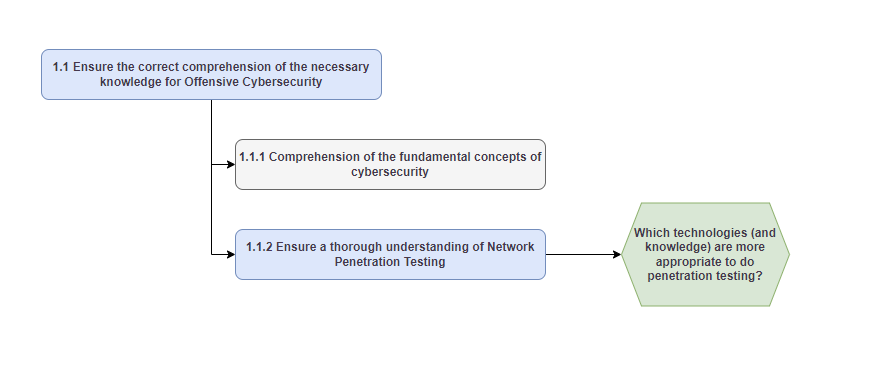
\includegraphics[width=\textwidth]{./assets/subgoal_1.1.2.png}
    \caption{Sub-Goal 1.1.2}
    \label{fig:subgoal_1.1.2}
\end{figure}

\begin{table}[H]
    \begin{center}
    \begin{tabular}{ | m{5cm} | m{5cm}| m{5cm} | } 
      \hline
      \textbf{Level 1 SA requirements} & \textbf{Level 2 SA requirements}  & \textbf{Level 3 SA requirements}  \\ 
      \hline
      Python operators & Cryptography techniques and hashing & Capability to choose the best penetration testing strategies based on the situation\\ 
      \hline
      Python syntax & Windows networking knowledge & \\ 
      \hline
      Powershell Scripting & Usage of variables & \\ 
      \hline
      Internet Protocol & Loops and functions in Python and Powershell  & \\ 
      \hline
      Domain Name System &  & \\ 
      \hline
    \end{tabular}
    \end{center}
    \caption{SA requirements for subgoal 1.1.2}
    \end{table}

\newpage
\subsection{Sub-Goal 1.1.3: Promote a solid understanding of SOC pratices and processes}
The objective of promoting a solid understanding of Security Operations Center (SOC) practices and processes is to provide individuals with the knowledge and skills necessary to effectively manage and respond to cybersecurity incidents. This includes foundational knowledge of network protocols such as the Internet Protocol (IP) and Domain Name System (DNS), as well as scripting skills with Powershell. Advanced competencies involve data conversion in Python between decimal, binary, and hexadecimal formats, understanding operational security and security management, and familiarity with practices such as the Cyber Kill Chain and logging. Ultimately, this comprehensive understanding enables individuals to proficiently detect and respond to cyber threats, ensuring robust security operations.

\begin{figure}[H]
    \centering
    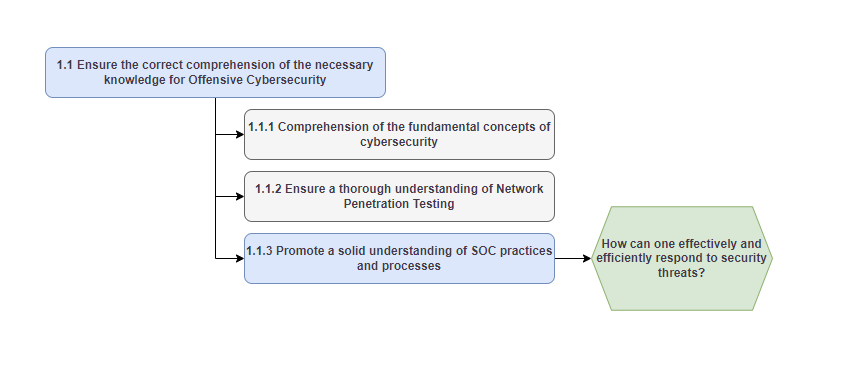
\includegraphics[width=\textwidth]{./assets/subgoal_1.1.3.png}
    \caption{Sub-Goal 1.1.3}
    \label{fig:subgoal1.1.3}
\end{figure}

\begin{table}[H]
\begin{center}
\begin{tabular}{ | m{5cm} | m{5cm}| m{5cm} | } 
  \hline
  \textbf{Level 1 SA requirements} & \textbf{Level 2 SA requirements}  & \textbf{Level 3 SA requirements}  \\ 
  \hline
  Internet Protocol & Data conversion in Python between decimal, binary, and hexadecimal & Knowing how to detect and respond to cyber threats\\ 
  \hline
  Powershell Scripting & Knowledge of operational security and security management & \\ 
  \hline
  Domain Name System & Practices of Cyber Kill Chain and Logging & \\ 
  \hline
  Firewall &  & \\ 
  \hline
\end{tabular}
\end{center}
\caption{SA requirements for subgoal 1.1.3}
\end{table}

\newpage
\subsection{Sub-Goal 1.1.4: Acquire advanced skills in Web Application Essentials}
The objective of acquiring advanced skills in web application essentials is to enable individuals to develop and maintain secure web applications. This encompasses foundational knowledge of web development technologies such as HTML, CSS, PHP, and JavaScript, along with proficiency in security tools like ZAP, AFL, SonarQube, and Flawfinder. Advanced skills include managing secure sessions, handling authentication, authorization, passwords, and cookies, and ensuring the security of REST, SOAP, and GraphQL services, as well as security practices in GIT. Ultimately, this comprehensive understanding equips individuals to recognize and mitigate vulnerabilities such as Server Side and Client Side XSS, Cross-Site Request Forgery, Clickjacking, and Content Sniffing, thereby ensuring robust web application security.

\begin{figure}[H]
    \centering
    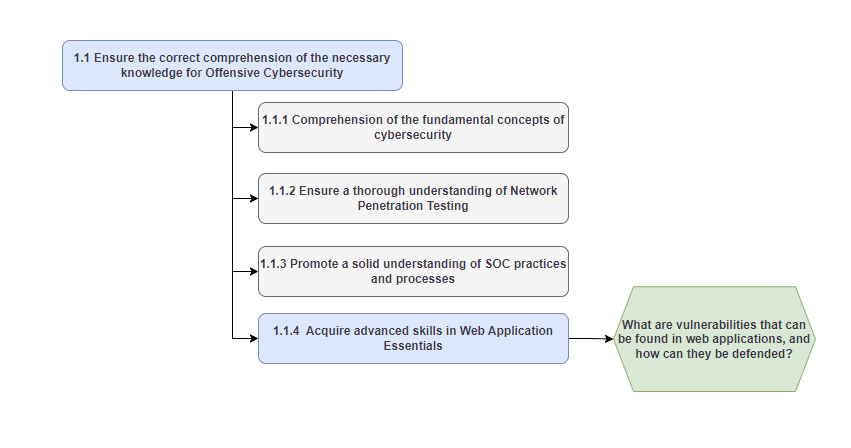
\includegraphics[width=\textwidth]{./assets/subgoal_1.1.4.png}
    \caption{Sub-Goal 1.1.4}
    \label{fig:subgoal1.1.4}
\end{figure}

\begin{table}[H]
\begin{center}
\begin{tabular}{ | m{5cm} | m{5cm}| m{5cm} | } 
  \hline
  \textbf{Level 1 SA requirements} & \textbf{Level 2 SA requirements}  & \textbf{Level 3 SA requirements}  \\ 
  \hline
  HTML, CSS, PHP, Javascript & Managing secure sessions, including authentication, authorization, passwords, and cookies, REST, SOAP and GraphQL services, security in GIT & Understanding how to make a secure web application\\ 
  \hline
  ZAP &  & Recognizing Server Side \& Client Side XSS, Cross-Site Request Forgery, Clickjacking, Content Sniffing\\ 
  \hline
  AFL &  & \\ 
  \hline
  SonarQube, Flawfinder &  & \\ 
  \hline
\end{tabular}
\end{center}
\caption{SA requirements for subgoal 1.1.4}
\end{table}

\newpage
\subsection{Sub-Goal 1.1.5: Demonstrate a solid proficiency in Exploit Development Essentials}
The objective of demonstrating solid proficiency in exploit development essentials is to enable individuals to effectively identify and develop exploits for various security vulnerabilities. This includes foundational knowledge of network protocols, VPNs, and firewalls. Advanced competencies involve understanding ARM-32 and ARM-64 assembly, manipulating registers, stacks, and functions, and analyzing binary files. Ultimately, this comprehensive skill set allows individuals to understand how malicious scripts affect applications, identify flaws in security measures, and leverage exploit frameworks to enhance cybersecurity defenses.

\begin{figure}[H]
  \centering
  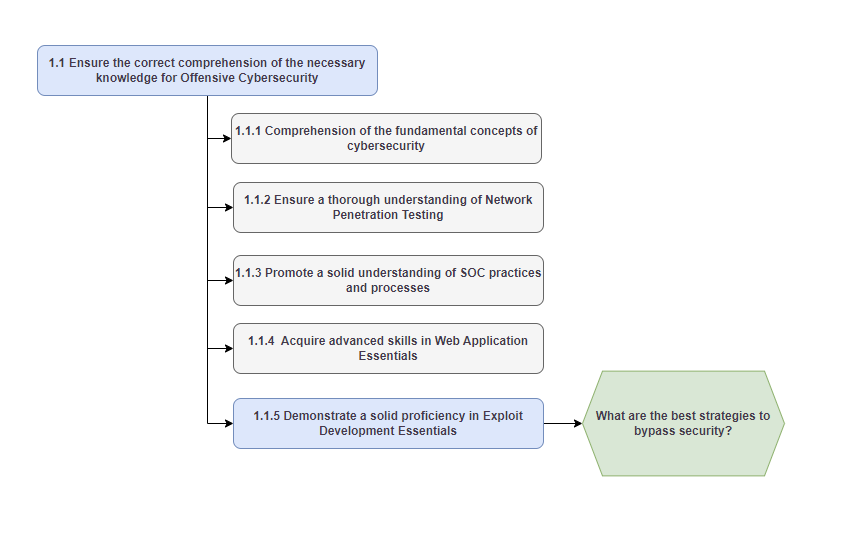
\includegraphics[width=\textwidth]{./assets/subgoal_1.1.5.png}
  \caption{Sub-Goal 1.1.5}
  \label{fig:subgoal1.1.5}
\end{figure}

\begin{table}[H]
    \begin{center}
    \begin{tabular}{ | m{5cm} | m{5cm}| m{5cm} | } 
      \hline
      \textbf{Level 1 SA requirements} & \textbf{Level 2 SA requirements}  & \textbf{Level 3 SA requirements}  \\ 
      \hline
      Network Protocols & Assembly for ARM-32 and ARM-64 & Understanding how a malicious script affects an application\\ 
      \hline
      VPN &  Registers, stacks and functions & Ability to identify flaws in security measures\\ 
      \hline
      Firewalls & Analysis of binary files & Knowledge of exploits frameworks\\  
      \hline
    \end{tabular}
    \end{center}
    \caption{SA requirements for subgoal 1.1.5}
    \end{table}

\newpage
\section{Major Goal 2.1: Ensure course optimization to maximize learning outcomes}
This Major-Goal aims to make the platform more engaging and effective for users. It focuses on two main things: boosting how users interact with the platform and making studying more personalized based on how each user learns.

To achieve this, the platform will track how users use it—what they're interested in, what skills they have, and where they might need help. With this info, the platform can adjust how it works to match each user's progress and preferences. 

\subsection{Sub-Goal 1.2.1: Improve student engagement with the platform}
The objective of improving student engagement with the platform focuses on increasing and enhancing student interactions. Key metrics include session length, number of active users, days spent on module, forum activity (questions and answers) and the engagement level with the platform. The analysis of these data involve user's session length compared with the length of other users session, a comparison between the days spent on a module by students, and student interaction within the forum. Ultimately, the goal is to prevent student dropout by understanding and addressing engagement factors.

\begin{figure}[H]
    \centering
    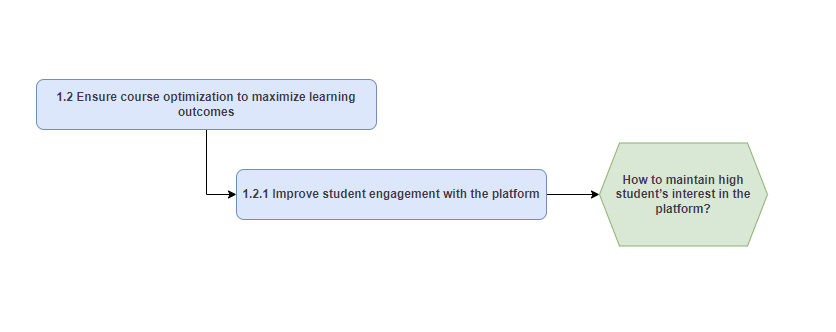
\includegraphics[width=\textwidth]{./assets/subgoal_1.2.1.png}
    \caption{Sub-Goal 1.2.1}
    \label{fig:subgoal1.2.1}
\end{figure}

\begin{table}[H]
\begin{center}
\begin{tabular}{ | m{5cm} | m{5cm}| m{5cm} | } 
  \hline
  \textbf{Level 1 SA requirements} & \textbf{Level 2 SA requirements}  & \textbf{Level 3 SA requirements}  \\ 
  \hline
  Number of active users &  Comparison between students session lengths & Preventing student dropout \\ 
  \hline
  Session length & Comparison between days spent on module by students & \\ 
  \hline
  Days spent on module & Student interaction within the forum & \\
  \hline
  Number of answers on the forum &  & \\ 
  \hline
  Number of questions on the forum &  & \\ 
  \hline
  Number of notifications on the forum &  & \\ 
  \hline
  Engagement Level & & \\ 
  \hline
\end{tabular}
\end{center}
\caption{SA requirements for subgoal 1.2.1}
\end{table}

\newpage
\subsection{Sub-Goal 1.2.2: Optimize student learning through personalization}
The objective of optimizing student learning through personalization is to enhance educational effectiveness by tailoring the learning experience to individual student needs and preferences. This involves assessing student performance through end-of-module assessments and tracking course completion. Additionally, it requires analyzing trends in student performance over time to identify areas for improvement. Furthermore, the initiative aims to optimize learning by monitoring the used resources, identifying areas of difficulty and preferred learning styles, and evaluating the acquisition of specific skills. By leveraging these insights, the goal is to create a more personalized educational environment that supports and enhances student learning outcomes effectively.
\begin{figure}[H]
    \centering
    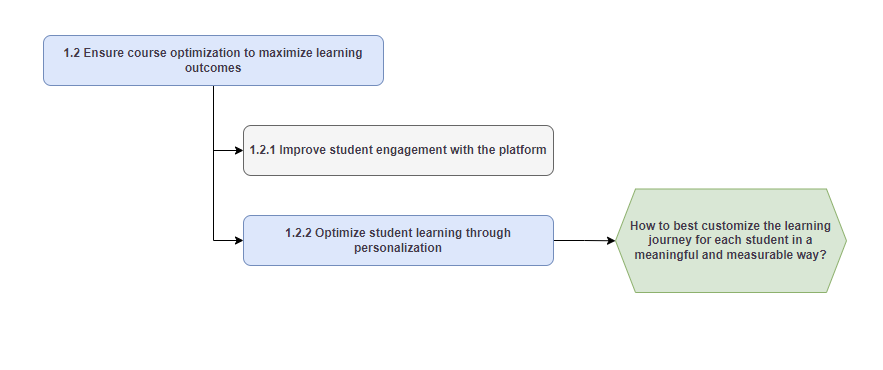
\includegraphics[width=\textwidth]{./assets/subgoal_1.2.2.png}
    \caption{Sub-Goal 1.2.2}
    \label{fig:subgoal1.2.2}
\end{figure}

\begin{table}[H]
\begin{center}
\begin{tabular}{ | m{5cm} | m{5cm}| m{5cm} | } 
  \hline
  \textbf{Level 1 SA requirements} & \textbf{Level 2 SA requirements}  & \textbf{Level 3 SA requirements}  \\ 
  \hline
  End-of-module test scores & Percentage of completed course & Trends in student performance over time \\ 
  \hline
  Modules visited & Problem-Solving vs Memory Performance & \\ 
  \hline
  Used material & Percentage of usage of the different kinds of materials provided to the students showing their preferences & \\ 
  \hline
   & Skill types and areas of difficulty & \\ 
  \hline
\end{tabular}
\end{center}
\caption{SA requirements for subgoal 1.2.2}
\end{table}

\chapter[Dashboard]{Dashboard}\label{ch:dashboard}
This paragraph will present the two dashboards implemented, the design principles used, and the SA demons that were tried to avoid. As mentioned before, to ensure that most of the requirements identified in the previous stage could be represented, it was decided to use a dataset entirely created by us to have full control over the data and its structure.

The whole system is divided into two dashboards, each associated with multiple goals. The first dashboard aims to establish \textbf{Common Operational Picture} that allows students to have an understanding of the current situation by integrating multiple subgoals into coherent visualizations. 
Unlike, the second dashboard, focuses on tracking and presenting student learning progress within a specific course.

\begin{itemize}
    \item \textbf{Dashboard I}: Subgoal 1.2.1 - Improve student engagement with the platform and Subgoal 1.2.2 - Optimize student learning through personalization.
    \item \textbf{Dashboard II}: Subgoal 1.1.1 - Comprehension of the fundamental concepts of cybersecurity, Subgoal 1.2.1 - Improve student engagement with the platform and Subgoal 1.2.2 - Optimize student learning through personalization.
\end{itemize} 

Both of the dashboards attempt to achieve the trade-off between supporting the operator's goal and supporting the overall SA. By placing the most important information appropriately at the center of each dashboard and positioning the supporting information on the sides, we ensure that relevant data is easily accessible to the student. This design choice is intended to reduce the cognitive load on the student, so he/she can quickly understand his current situation and make informed decisions about his learning path.

Some common guidelines were used to blend the student experience and create a sense of confidence in switching between the different dashboards and to enhance efficiency by transporting the experience matured in one dashboard to the other. This is helpful so that the student can create expectations about the interface, increasing his or her satisfaction.

\section{Dashboard I}

The objectives of this dashboard are to maintain student engagement with the platform and to assist in tailoring the learning process to meet the student's needs.

To ensure the student is aware that he/she are on the home page of the platform, the name of the platform \textbf{OffSec} is included, representing \textit{Offensive Cybersecurity}. Additionally, a "Welcome Marta!" message is displayed to emphasize that this dashboard is the home page. These two elements help prevent the student from using an incorrect mental model when interpreting the dashboard's components, effectively avoiding the \textbf{Wrong Mental Model} demon.

\begin{figure}[H]
    \centering
    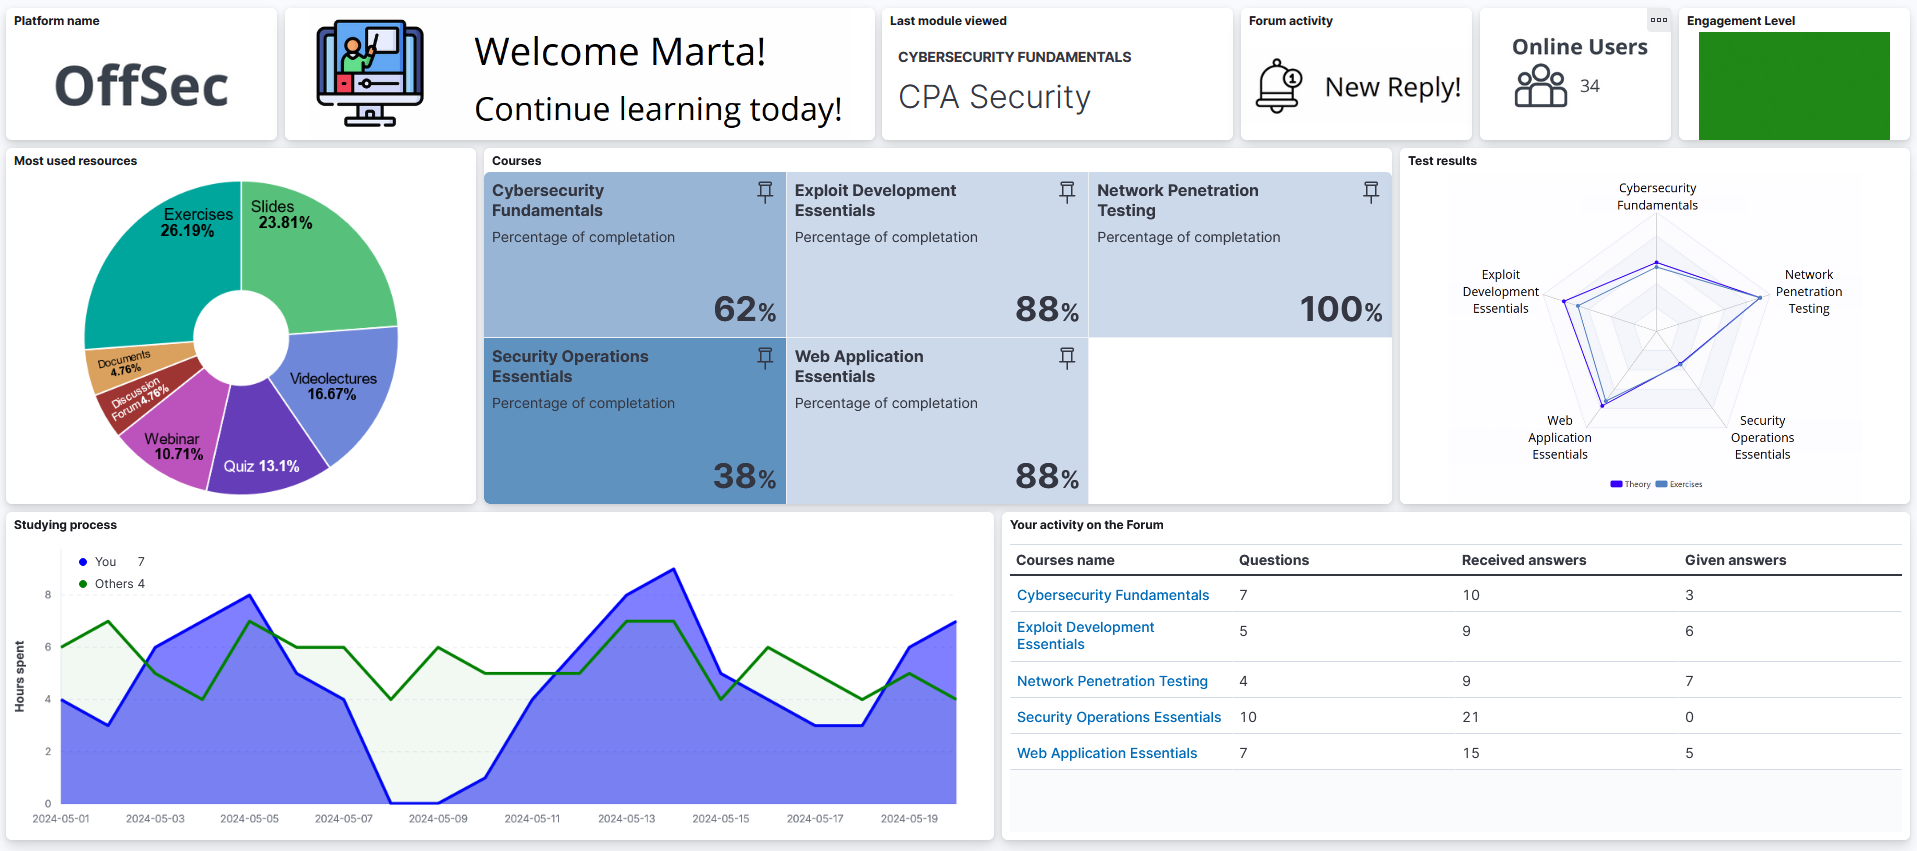
\includegraphics[width=0.9\textwidth]{assets/dashboard_1.png}
    \caption{Dashboard I}
    \label{fig:dashboard_1}
\end{figure}

To ensure compliance with \textbf{Design Principle 4} and in order to support \textbf{Design Principle 1}, the dashboard should be designed with central elements supporting specific goals, 
surrounded by elements that provide an overview of the student's progress. But typically, e-learning systems display an overview of the courses the student is following. 
Therefore, we adopted this common approach for our system as well.
As shown in Figure 6.1, the center of the screen features a matrix of the various courses the student needs to complete for upskilling, 
with each course's completion percentage clearly indicated. This allows students to quickly understand his/her progress, supporting his/her 
overall SA.

This design choice supports both \textbf{Design Principle 5 and Design Principle 6} through the effective use of salience. 
Darker colors in the matrix highlights courses with lower completion percentages, drawing the student's attention to these areas and guiding the student towards the courses that need more
attention before his/her deadlines. This can prompt a shift from data-driven to goal-driven behavior, encouraging the student to prioritize completing the less finished courses. 

In order to form the right Global SA of the student, on 
the right side of the screen there is a spider chart showing the results of the student on theoretical tests and
practical tests, weighted on the number of tests completed for the course.
Instead, on the left side of the screen, there is a
donut chart, that shows which resources the student has preferred for the different courses 
the student has used, in order to support the \textbf{Subgoal 1.2.2}.

The linear graph, which shows the student's time spent on the platform since the start of the upskilling process, supports \textbf{Subgoal 1.2.1}. 
It allows the student to compare his/her time spent on the platform with the time spent by other students. 
By observing this graph, the student can become aware of his/her own hours invested. 
If the student notices that other students have spent significantly more time on the platform, it can serve as a motivation for him/her to dedicate more time to the learning process. 
This comparative visualization encourages students to increase his/her engagement and commitment to the platform, cultivating a more competitive and driven learning environment.


\begin{figure}[H]
    \centering
    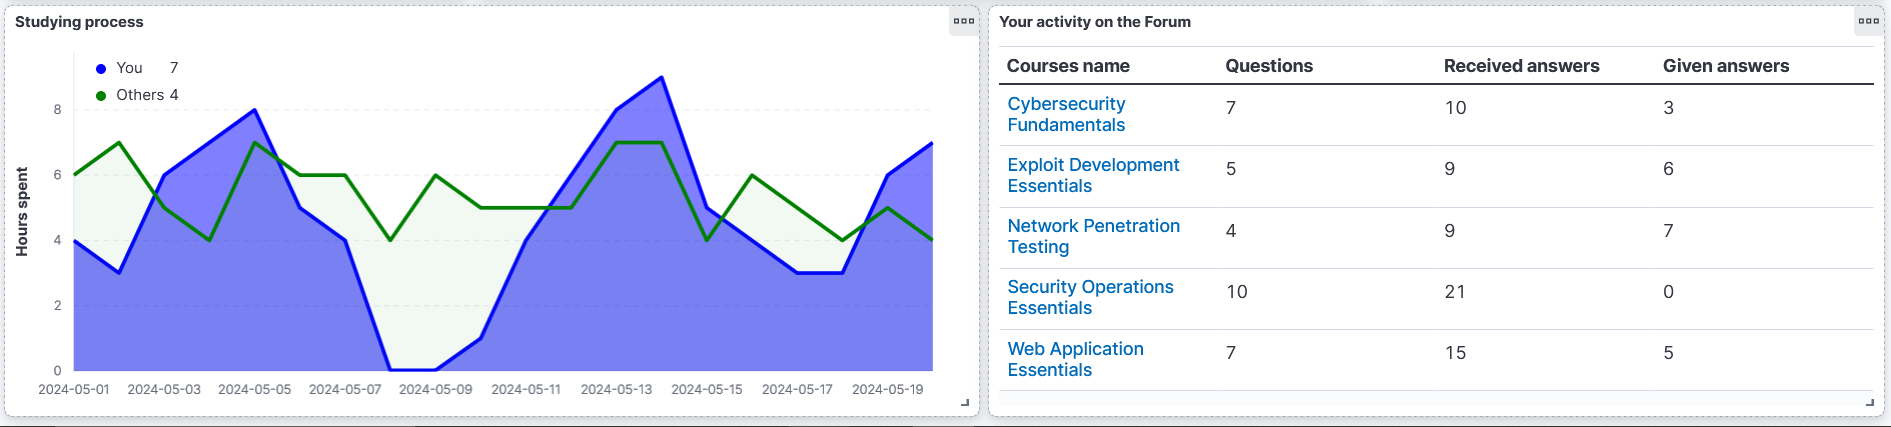
\includegraphics[width=0.9\textwidth]{assets/dashboard_1_121.png}
    \caption{Dashboard I - Subgoal 1.2.1}
    \label{fig:dashboard_1_subgoal_121}
\end{figure}

The elements present in Figure 6.3 indicate student engagement with the platform, presenting (from right to left) the computed engagement level using the CST described in a previous chapter, the number of students currently online, a notifications section from the forum, and an element displaying the last viewed module. Together, these components maintain continuous global situational awareness to prevent the occurrence of the \textbf{Attentional Tunneling} demon.
In particular, the last viewed module element helps to avoid the \textbf{Memory Trap} demon by providing a quick reminder of the student's most recent activity, reducing the cognitive load associated with remembering the last module he/she accessed.

\begin{figure}[H]
    \centering
    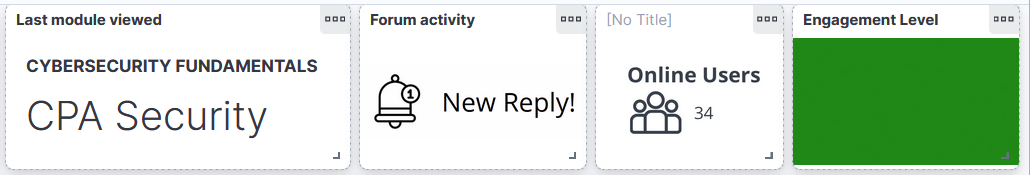
\includegraphics[width=0.9\textwidth]{assets/dashboard_1_globaltop.png}
    \caption{Dashboard I - Global Top}
    \label{fig:dashboard_1_global_top}
\end{figure}

Given that human attention and working memory are limited, most of the information has been processed and integrated in terms of Level 2 SA, supporting comprehension. Therefore, \textbf{Design Principle 2} has been satisfied.
This allowed us to avoid the \textbf{Memory Trap} demon, which can occur when students are required to remember too much information. 
Moreover, the use of visualizations such as the spider chart and the donut chart helps to avoid the \textbf{Data Overload} demon and the \textbf{Complexity Creep} demon, as he/she provide a more compact representation of the data, reducing the amount of information that needs to be processed.

Another element that could contribute to support the \textbf{Design Principle 5} is the presence of the notifications from the forum, which can capture the student's attention and facilitate the switch between goal-driven and data-driven processing. This element helps to avoid the \textbf{Attentional Tunneling} demon.

The engagement level element is displayed as a square shape filled with a color, which can capture the student's attention when it is not needed, causing a bit of the \textbf{Misplaced Salience} demon. 
Though, the use of colors (green, yellow, orange) suggests that if the indicator is green, the student's attention may briefly focus on it, indicating satisfaction or a certain level of confidence in his/her engagement level. Unlike the yellow and orange colors that might encourage the student to spend more time on the platform and interact more actively with it.

The dashboard effectively prevents the \textbf{Out of the Loop} demon since there are no autonomous functions that operate independently and since it is crucial for the student to make decisions about his/her actions and timing autonomously.

Our goal is also to fulfill \textbf{Design Principle 3}, which emphasizes providing Level 3 assistance. 
This is facilitated within our dashboard through the inclusion of a forum. By interacting with other students to discuss course-related 
questions and challenges, students can obtain answers and support. This interaction could encourage them to continue his/her learning journey, 
thereby reducing the likelihood of abandoning the platform. 

\section{Dashboard II}

The goal of the dashboard is to support the student's learning process within a specific course. It is characterized by the title \textbf{Cybersecurity Fundamentals} to indicate the course the student is currently focusing on. The inclusion of a specific course title on the dashboard plays a crucial role in preventing student confusion, especially given the variety of courses a student might be enrolled in. 
In this way, it mitigates the risk of the \textbf{Wrong Mental Model} demon, ensuring that students maintain an accurate understanding of his/her learning progress and requirements within the context of the specific course he/she are viewing. 

The choice of different data visualizations used made it possible to reduce the effects of the \textbf{Data Overload} demon as well, by being able to convey the information by expressing it in graphical form rather than in textual or tabular form (e.g., pie charts for the most used resources), reducing the cognitive load on the student. 

A first view of the second dashboard is shown in the following figure.

\begin{figure}[H]
    \centering
    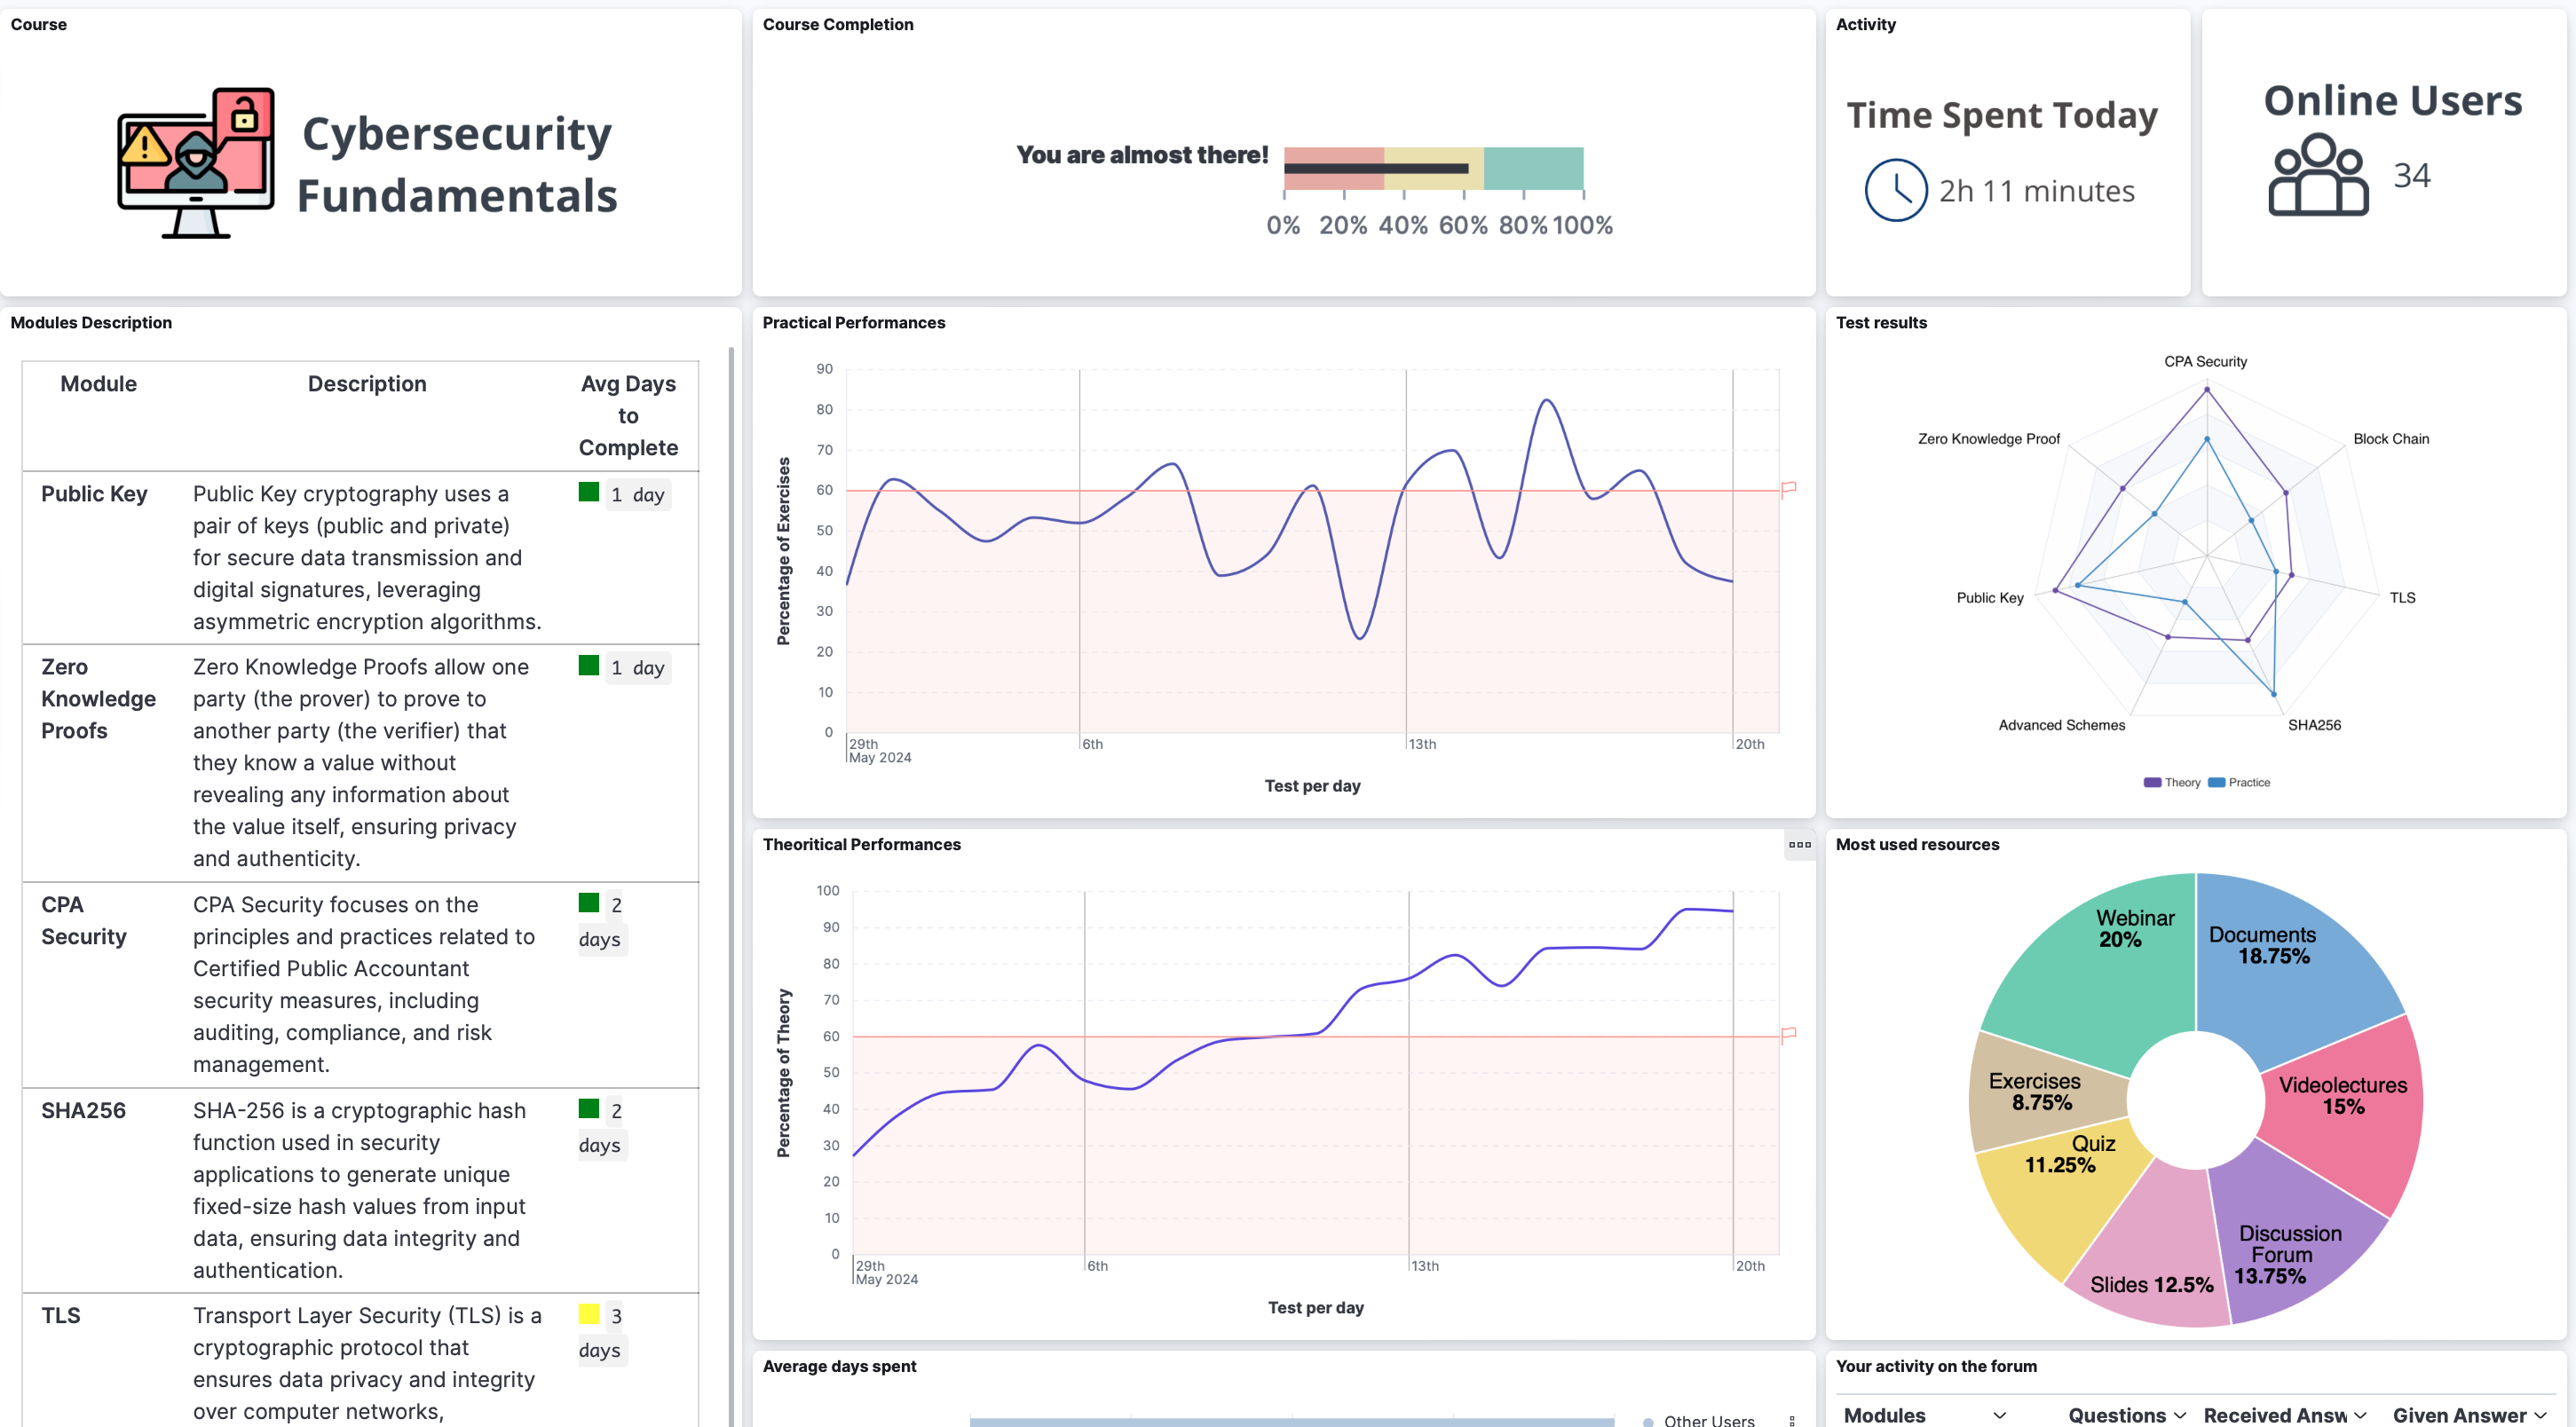
\includegraphics[width=0.9\textwidth]{assets/dashboard_2.png}
    \caption{Dashboard II}
    \label{fig:dashboard_2}
\end{figure}

With multiple subgoals active on the dashboard, it’s important that when a student opens it, he/she can quickly figure out the necessary information to achieve his/her objectives. 

This follows \textbf{Design Principle 1}, which ensures that information is provided effectively to support decision-making. When a student clicks on a course, he/she will see two line charts in the center of the dashboard showing his/her progress and the course completion status.

These charts, like the others on the dashboard, also satisfy \textbf{Design Principle 2} because the interface provides already processed and integrated information at Level 2. Specifically, the Level 2 and Level 1 data allow for a complete understanding of the situation, such as the student's performances in the course, without the need for further processing.

To ensure that salience is appropriately balanced within the dashboard, the latter is placed only on information considered important. For instance, the red threshold line in the main charts indicates that if a student's end-of-module test scores fall below 60\%, he/she needs to decide on a strategy for improvement. Hence, this visual cue helps students understand that he/she should aim for scores above this threshold.

The two line charts, also support \textbf{Design Principle 3} by providing level 3 projection assistance. This means that if a student maintains consistent performance across multiple modules, it can be projected that he/she will likely perform well in future modules. 

\begin{figure}[H]
    \centering
    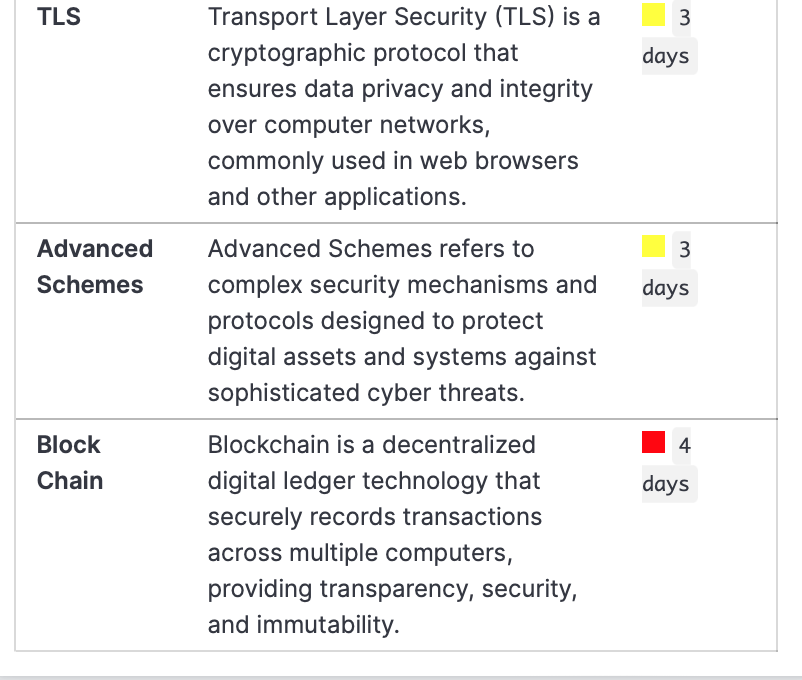
\includegraphics[width=0.3\textwidth]{assets/descriptionmodule.png}
    \caption{Dashboard II - Progress}
    \label{fig:dashboard_2} 
\end{figure}

As we can see in Figure 6.5, the estimated completion days for each module, within the section where the modules are listed with their description, are highlighted in red if they exceed four days, based on data from previous students who have taken the course. This alerts the student that it may be necessary to put in more effort for these particular modules.
The use of red to draw attention to critical areas complies with \textbf{Design Principle 6}, clearly signaling to the student where he/she needs to focus and prompting him/her to take corrective action if necessary.

The dashboard also includes a gauge chart dedicated to overall course completion. If a student has completed less than 40\% of the course, this chart will highlight the need for increased attention to ensure timely course completion.
The addition of a course completion chart helps reduce the cognitive load on the student by offering a visual depiction of his/her progress. This feature was intentionally introduced to prevent the student from having to remember the completion percentage shown on the main dashboard and to overcome relying on memory (facing the \textbf{Memory Trap} demon), which can often not guarantee accurate awareness and decision-making.

Given that the dashboard supports three subgoals, it is likely that when a student first opens the dashboard for a specific course, it will be done to check his/her progress. 

Through various charts—such as those showing the theoretical and practical test performance, course completion status, and average grades, he/she can assess the level of understanding of the course. 
These elements also supports the subgoal related to optimizing learning through personalization, including a pie chart that shows the usage of different learning materials for each module in order to show his/her learning preferences. 

\begin{figure}[H]
    \centering
    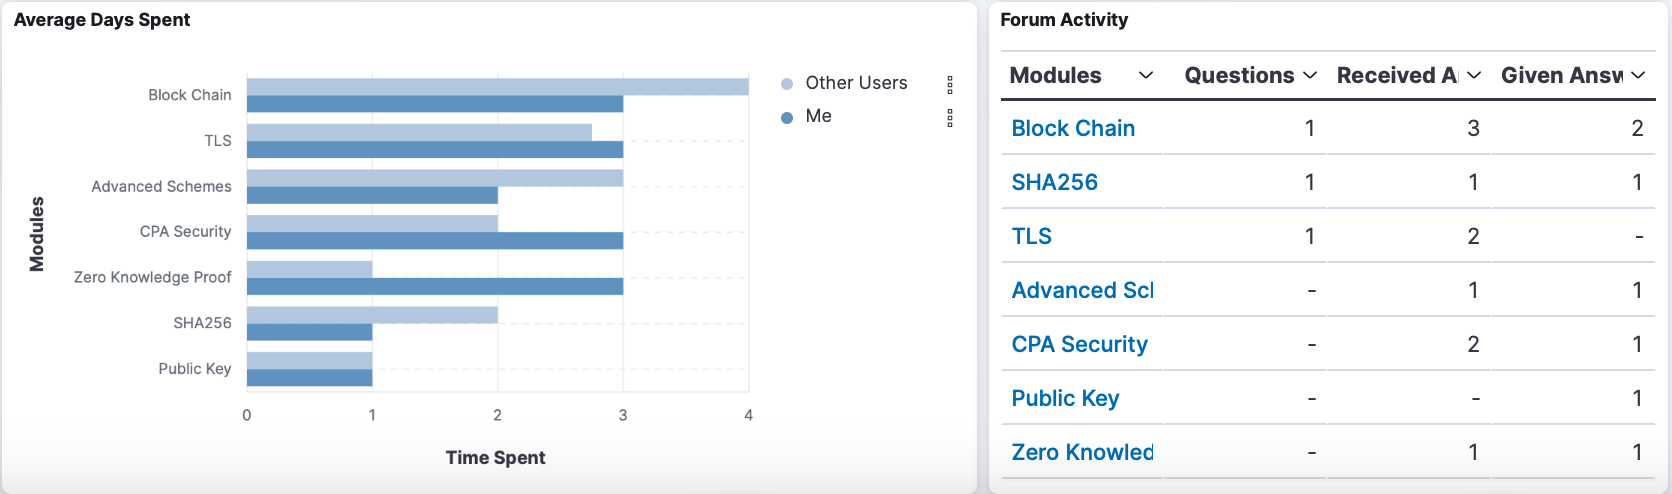
\includegraphics[width=0.9\textwidth]{assets/forum2.png}
    \caption{Dashboard II - Forum}
    \label{fig:dashboard_2}
\end{figure}

\begin{figure}[H]
    \centering
    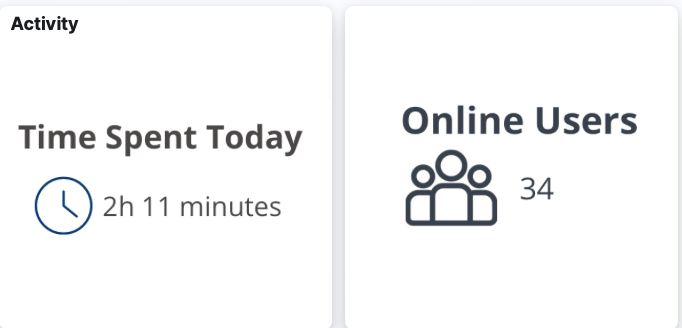
\includegraphics[width=0.3\textwidth]{assets/activity2.png}
    \caption{Dashboard II - Student Activity}
    \label{fig:dashboard_2}
\end{figure}

The elements in Figure 6.6 and 6.7 support goals related to engagement with the platform such as activities in the forum, the number of students online at the time of access, the time spent on the platform, and the days taken to complete each module compared to other students.

Therefore, we assume that at first glance, the student decides to focus on the first subgoal \textbf{Comprehension of the fundamental concepts of cybersecurity} to reach his/her objective and then potentially switches to other supported goals as he/she shifts the attention to the other charts. This approach could satisfy \textbf{Design Principle 5 and Design Principle 4} by including elements in the dashboard that capture attention on aspects satisfying different goals. This prevents attention from being confined to a limited set of information, thereby overcoming the issue of \textbf{Attentional Tunneling} demon and supporting the switch between goal-driven and data-driven modes based on the goal the student wishes to achieve.



\chapter[Conclusions]{Conclusions}\label{ch:conclusions}




\setcounter{page}{1}
\pagenumbering{roman}
% \tableofcontents


\listoffigures
\listoftables
%\printbibliography

\end{document}
